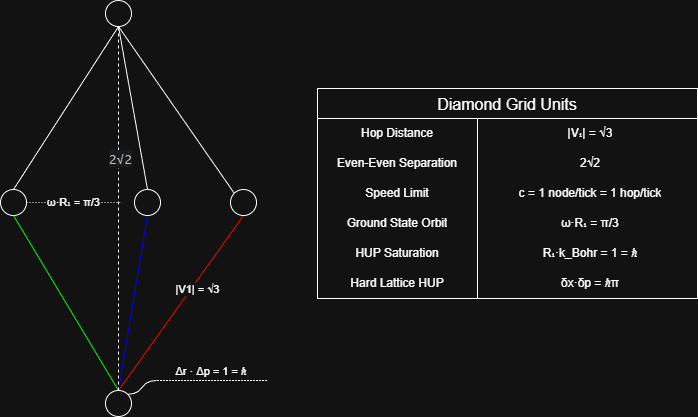
\includegraphics[width=0.85\textwidth]{../figures/Diamond_Grid_Units_drawio.png}
\caption{\small Fundamental length and momentum scales of the $\Tdiamond$
lattice.
\textbf{Hop distance.}
Every propagation step moves a spinor amplitude along one of the six basis
vectors $\mathbf{V}_i$; the shortest is $|\mathbf{V}_1| = |(1,1,1)| = \sqrt{3}$
grid units, which sets the natural length unit $h \equiv \sqrt{3}\,\ell_P$
(one body-diagonal of the unit cube).
\textbf{Same-sublattice exclusion.}
Even (RGB) nodes are separated from their nearest even neighbours by
$|2\mathbf{V}_1 - 2\mathbf{V}_2| = 2\sqrt{2}\,\ell_P$ --- a face-diagonal
distance that no two same-chirality particles can reduce below without
violating the bipartite tick rule.
This geometric floor is the lattice analogue of the Pauli exclusion
principle: same-sublattice occupation is forbidden by structure, not by
postulate.
\textbf{Speed limit.}
A massless session ($\omega = 0$, $p_\text{stay} = 0$) hops every tick
without ever residing, giving $c = 1$ node/tick $= 1$ hop/tick, confirmed
by \texttt{exp\_00}.
\textbf{Uncertainty product.}
The hard lattice spacing sets $\delta x \cdot \delta p = \hbar\pi$, above
the Gaussian minimum $\hbar/2$ but consistent with a discrete Brillouin-zone
cutoff at $|p| = \pi/\sqrt{3}$.
\textbf{Ground-state saturation.}
The Bohr orbit satisfies $R_1 \cdot k_\text{Bohr} = R_1 \cdot (1/R_1) = 1
= \hbar$ (lattice units), making the $n=1$ orbital the minimum-uncertainty
state: $\Delta r \cdot \Delta p = 1 \geq \tfrac{1}{2}$.
\textbf{Arnold tongue identity.}
The simulation recovers $\omega \cdot R_1 \approx \pi/3$ to $0.23\%$ at
$\omega = 0.1019$, STRENGTH $= 30$ --- a dynamical result, not a geometric
identity.
This is the 3:1 Zitterbewegung/orbital resonance (lowest Arnold tongue of
the ground state); it is to be derived from the continuum limit, not assumed.
\textbf{Calibration summary (lattice units, $\hbar = c = 1$).}
$\delta x = \sqrt{3}\,\ell_P$;\
$c = 1$ hop/tick;\
$\delta x \cdot \delta p = \hbar\pi^*$;\
$R_1 \cdot k_\text{Bohr} = 1^{\ddagger}$;\
$\omega \cdot R_1 = \pi/3^{\dagger}$.
\newline
\footnotesize
$^*$Brillouin-zone floor\quad
$^\ddagger$\texttt{exp\_12} two-body hydrogen\quad
$^\dagger$\texttt{exp\_11}/\texttt{exp\_12} 3:1 Arnold tongue.}
